% Week 6: Pre-trained Language Models - Pedagogical Version
% NLP Course 2025
% Created: 2025-09-30 01:00

\documentclass[8pt,aspectratio=169]{beamer}
\usetheme{Madrid}
\usecolortheme{default}
\setbeamertemplate{navigation symbols}{}

% Lavender color scheme from template_beamer_final
\definecolor{mllavender}{RGB}{200,180,220}
\definecolor{mlpurple}{RGB}{130,100,160}
\definecolor{mlblue}{RGB}{100,120,180}
\definecolor{mldarkblue}{RGB}{60,80,120}
\definecolor{mlgray}{RGB}{100,100,100}

% Apply the lavender color scheme
\setbeamercolor{structure}{fg=mlpurple}
\setbeamercolor{frametitle}{bg=mllavender!70,fg=mldarkblue}
\setbeamercolor{title}{fg=mldarkblue}
\setbeamercolor{subtitle}{fg=mlpurple}
\setbeamercolor{author}{fg=mlgray}
\setbeamercolor{date}{fg=mlgray}
\setbeamercolor{block title}{bg=mllavender!50,fg=mldarkblue}
\setbeamercolor{block body}{bg=mllavender!10}

% Custom commands
\newcommand{\highlight}[1]{\textcolor{mlpurple}{\textbf{#1}}}
\newcommand{\keypoint}[1]{
    \vspace{2mm}
    \begin{center}
    \colorbox{mllavender!30}{\parbox{0.9\textwidth}{\centering\small #1}}
    \end{center}
    \vspace{2mm}
}
\newcommand{\warning}[1]{\textcolor{red!70!black}{\textbf{Warning:} #1}}
\newcommand{\success}[1]{\textcolor{green!70!black}{\textbf{#1}}}
\newcommand{\secondary}[1]{\textcolor{mlgray}{#1}}
\newcommand{\formula}[1]{
    \begin{center}
    \colorbox{mllavender!20}{\parbox{0.8\textwidth}{\centering\large $\displaystyle #1$}}
    \end{center}
}

% Bottom note command
\newcommand{\bottomnote}[1]{
    \vfill
    \begin{center}
    \textcolor{mlgray}{\footnotesize\textit{#1}}
    \end{center}
}

% Checkpoint command for pedagogical approach
\newcommand{\checkpoint}[1]{
    \begin{center}
    \colorbox{yellow!30}{\parbox{0.9\textwidth}{\centering\small\textbf{#1}}}
    \end{center}
}

% Pedagogical boxes
\newcommand{\intuition}[1]{
    \begin{center}
    \colorbox{purple!10}{\parbox{0.9\textwidth}{\small\textbf{Intuition:} #1}}
    \end{center}
}

\newcommand{\realworld}[1]{
    \begin{center}
    \colorbox{orange!10}{\parbox{0.9\textwidth}{\small\textbf{Real World:} #1}}
    \end{center}
}

\newcommand{\misconception}[1]{
    \begin{center}
    \colorbox{red!10}{\parbox{0.9\textwidth}{\small\textbf{Common Misconception:} #1}}
    \end{center}
}

% Code listing setup
\usepackage{listings}
\lstset{
    basicstyle=\tiny\ttfamily,
    keywordstyle=\color{mlblue},
    commentstyle=\color{mlgray},
    frame=single,
    backgroundcolor=\color{mllavender!10},
    numbers=left,
    numberstyle=\tiny\color{mlgray}
}

% Packages
\usepackage{amsmath,amssymb}
\usepackage{graphicx}
\usepackage{tikz}
\usepackage{pgfplots}
\pgfplotsset{compat=1.17}
\usepackage{tcolorbox}
\tcbuselibrary{skins}

\title{Pre-trained Language Models}
\subtitle{Chapter 6: Learning from All of Human Knowledge}
\author{NLP Course 2025}
\date{\today}

\begin{document}

% Title slide
\begin{frame}
\titlepage
\vfill
\begin{center}
\secondary{\footnotesize A pedagogical journey from wasteful repetition to efficient transfer learning}\\
\secondary{\footnotesize 45 slides • 4 sections • 2 checkpoints}
\end{center}
\end{frame}

% Learning objectives
\begin{frame}{Your Learning Journey Today}
\begin{center}
{\Large \textbf{What You Will Master}}
\end{center}

\vspace{8mm}

\begin{columns}[T]
\column{0.48\textwidth}
\textbf{Conceptual Understanding}
\begin{itemize}
\item Why pre-training revolutionized NLP
\item Transfer learning principles
\item BERT vs GPT paradigms
\item Fine-tuning strategies
\item Model selection criteria
\end{itemize}

\column{0.48\textwidth}
\textbf{Practical Skills}
\begin{itemize}
\item Use pre-trained models
\item Fine-tune for your task
\item Choose the right model
\item Implement with HuggingFace
\item Avoid common pitfalls
\end{itemize}
\end{columns}

\vspace{8mm}
\keypoint{By the end: You'll understand how to leverage billions of parameters trained on terabytes of text}

\bottomnote{Pre-training changed everything - from months to minutes, from millions to thousands}
\end{frame}

% ============================================
% SECTION 1: THE CHALLENGE
% ============================================

\section{The Challenge: Reinventing the Wheel}

% Section title slide
\begin{frame}
\begin{center}
{\Huge \textbf{Section 1}}\\
\vspace{5mm}
{\Large The Challenge}\\
\vspace{10mm}
{\large Reinventing the Wheel}
\end{center}
\end{frame}

% The Reading Revolution Story
\begin{frame}{The Reading Revolution: An Analogy}
\textbf{Imagine two medical students:}

\vspace{8mm}
\begin{columns}[T]
\column{0.48\textwidth}
\textbf{Student A: Starting from Zero}
\begin{itemize}
\item Never learned to read
\item Must learn alphabet first
\item Then words, grammar, sentences
\item Finally can read medical texts
\item Takes 10 years to become doctor
\end{itemize}

\vspace{5mm}
\warning{90\% of time learning to read, only 10\% on medicine}

\column{0.48\textwidth}
\textbf{Student B: Transfer Learning}
\begin{itemize}
\item Already knows how to read
\item Starts directly with medical texts
\item Focuses only on medical knowledge
\item Becomes doctor in 4 years
\item Better outcomes, less time
\end{itemize}

\vspace{5mm}
\success{100\% of time on medicine, reading skill transfers}
\end{columns}

\vspace{8mm}
\intuition{Pre-training is like teaching AI to read before teaching it specific tasks!}

\bottomnote{This analogy captures why pre-training changed everything in NLP}
\end{frame}

% The Million Dollar Problem
\begin{frame}{The \$10 Million Problem No One Talked About}
\textbf{The wasteful reality of 2017-2018:}

\vspace{8mm}
\begin{columns}[T]
\column{0.48\textwidth}
\textbf{The Old Way:}
\begin{itemize}
\item Company A: Sentiment analysis
\begin{itemize}
\item Cost: \$500,000
\item Time: 2 weeks on 64 GPUs
\item Learns: Grammar from scratch
\end{itemize}
\item Company B: Translation
\begin{itemize}
\item Cost: \$500,000
\item Time: 2 weeks on 64 GPUs
\item Learns: Grammar from scratch
\end{itemize}
\item Company C: Q\&A
\begin{itemize}
\item Cost: \$500,000
\item Time: 2 weeks on 64 GPUs
\item Learns: Grammar from scratch
\end{itemize}
\end{itemize}

\vspace{3mm}
\textbf{Total waste: \$1.5 million!}

\column{0.48\textwidth}
\textbf{The Smart Way (Today):}
\begin{itemize}
\item Pre-train ONCE: \$1 million
\item Fine-tune for each task:
\begin{itemize}
\item Sentiment: \$10,000
\item Translation: \$10,000
\item Q\&A: \$10,000
\end{itemize}
\end{itemize}

\vspace{8mm}
\textbf{Total cost: \$1.03 million}\\
\textbf{Savings: \$470,000!}

\vspace{5mm}
\success{Plus: Better performance!}
\end{columns}

\vspace{8mm}
\keypoint{Every team was re-learning what ``the`` means from scratch!}

\bottomnote{These numbers are real - based on 2018 cloud compute costs}
\end{frame}

% What Models Learn Repeatedly
\begin{frame}{What Every Model Was Learning from Scratch}
\textbf{The redundant learning pyramid:}

\vspace{8mm}
\begin{center}
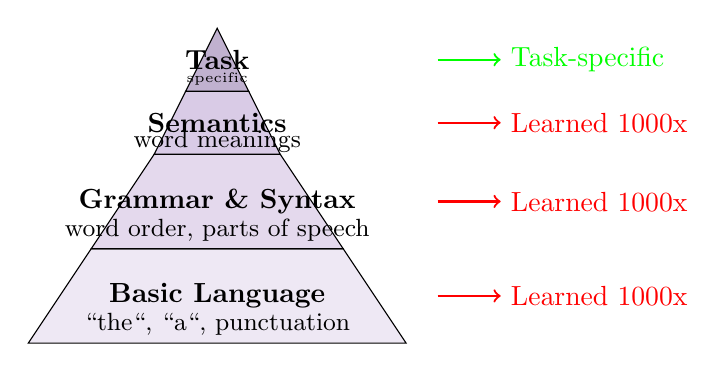
\begin{tikzpicture}[scale=0.8]
% Pyramid layers
\draw[fill=mllavender!30] (0,0) -- (6,0) -- (5,1.5) -- (1,1.5) -- cycle;
\draw[fill=mllavender!50] (1,1.5) -- (5,1.5) -- (4,3) -- (2,3) -- cycle;
\draw[fill=mllavender!70] (2,3) -- (4,3) -- (3.5,4) -- (2.5,4) -- cycle;
\draw[fill=mlpurple!50] (2.5,4) -- (3.5,4) -- (3,5) -- cycle;

% Labels
\node at (3,0.75) {\textbf{Basic Language}};
\node at (3,0.3) {\small ``the``, ``a``, punctuation};
\node at (3,2.25) {\textbf{Grammar \& Syntax}};
\node at (3,1.8) {\small word order, parts of speech};
\node at (3,3.5) {\textbf{Semantics}};
\node at (3,3.2) {\small word meanings};
\node at (3,4.5) {\textbf{Task}};
\node at (3,4.2) {\tiny specific};

% Arrows showing waste
\draw[->, thick, red] (6.5,0.75) -- (7.5,0.75) node[right] {Learned 1000x};
\draw[->, thick, red] (6.5,2.25) -- (7.5,2.25) node[right] {Learned 1000x};
\draw[->, thick, red] (6.5,3.5) -- (7.5,3.5) node[right] {Learned 1000x};
\draw[->, thick, green] (6.5,4.5) -- (7.5,4.5) node[right] {Task-specific};
\end{tikzpicture}
\end{center}

\vspace{8mm}
\misconception{``Each task needs its own model from scratch'' - False! 95\% of language understanding is general}

\bottomnote{The bottom 95\% of the pyramid is identical for all NLP tasks}
\end{frame}

% Computational Cost Visualization
\begin{frame}{The Computational Reality}
\textbf{Training costs over time:}

\vspace{5mm}
\begin{center}
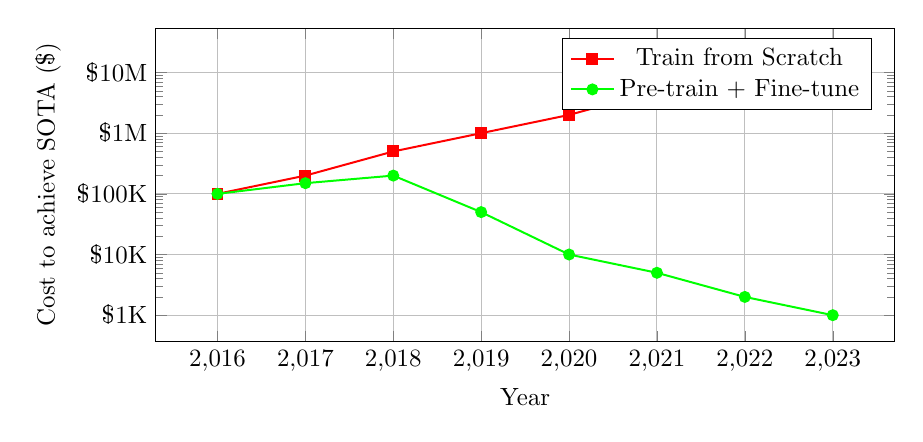
\begin{tikzpicture}[scale=0.9]
\begin{axis}[
    xlabel={Year},
    ylabel={Cost to achieve SOTA (\$)},
    ymode=log,
    width=12cm,
    height=6cm,
    grid=major,
    legend pos=north east,
    xtick={2016,2017,2018,2019,2020,2021,2022,2023},
    ytick={1000,10000,100000,1000000,10000000},
    yticklabels={\$1K,\$10K,\$100K,\$1M,\$10M}
]

% From scratch line
\addplot[color=red, thick, mark=square*] coordinates {
    (2016, 100000)
    (2017, 200000)
    (2018, 500000)
    (2019, 1000000)
    (2020, 2000000)
    (2021, 5000000)
    (2022, 10000000)
    (2023, 20000000)
};

% Pre-training + fine-tuning line
\addplot[color=green, thick, mark=*] coordinates {
    (2016, 100000)
    (2017, 150000)
    (2018, 200000)
    (2019, 50000)
    (2020, 10000)
    (2021, 5000)
    (2022, 2000)
    (2023, 1000)
};

\legend{Train from Scratch, Pre-train + Fine-tune}
\end{axis}
\end{tikzpicture}
\end{center}

\vspace{5mm}
\keypoint{Pre-training inverted the cost curve - better models got cheaper!}

\bottomnote{The divergence started with BERT in 2018}
\end{frame}

% Environmental Impact
\begin{frame}{The Carbon Footprint Reality}
\textbf{Environmental cost of training:}

\vspace{8mm}
\begin{columns}[T]
\column{0.48\textwidth}
\textbf{Training from Scratch (per model):}
\begin{itemize}
\item Energy: 27,000 kWh
\item CO2: 12 metric tons
\item Equivalent to:
\begin{itemize}
\item 5 cars for 1 year
\item 125 flights NYC-SF
\item Average home for 2.5 years
\end{itemize}
\end{itemize}

\vspace{5mm}
\textbf{If 1000 companies do this:}
\begin{itemize}
\item 12,000 metric tons CO2
\item Small city's annual emissions
\end{itemize}

\column{0.48\textwidth}
\textbf{Pre-training + Fine-tuning:}
\begin{itemize}
\item Pre-train once: 12 metric tons
\item Fine-tune: 0.01 metric tons
\item 1000 companies: 22 metric tons total
\end{itemize}

\vspace{5mm}
\success{545x reduction in carbon footprint!}

\vspace{5mm}
\begin{center}
% \includegraphics[width=0.8\textwidth]{../figures/carbon_footprint.pdf}
\textit{[Carbon footprint visualization]}
\end{center}
\end{columns}

\vspace{8mm}
\realworld{Google's BERT pre-training saved an estimated 50,000 metric tons of CO2}

\bottomnote{Environmental responsibility drove adoption as much as cost savings}
\end{frame}

% The Transfer Learning Opportunity
\begin{frame}{The Transfer Learning Opportunity}
\textbf{What if we could share knowledge?}

\vspace{8mm}
\begin{center}
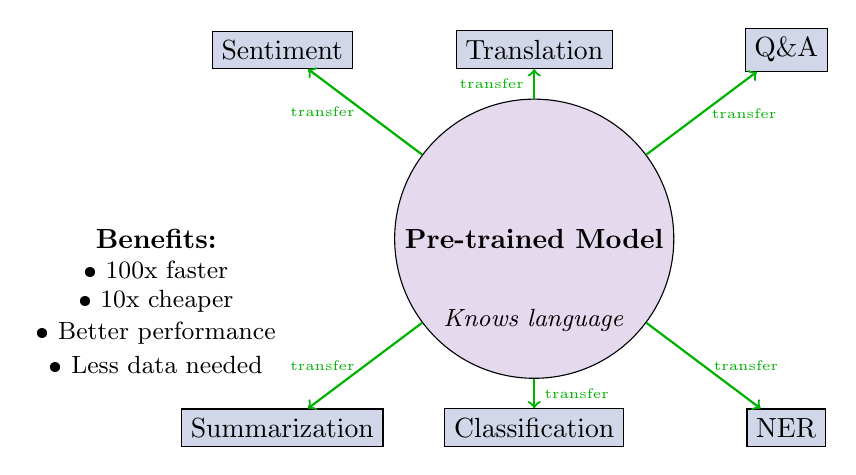
\begin{tikzpicture}[scale=0.8]
% Central pre-trained model
\node[circle, draw, fill=mllavender!50, minimum size=2cm] (center) at (0,0) {\textbf{Pre-trained Model}};
\node at (0,-1.3) {\small \textit{Knows language}};

% Task-specific models around it
\node[rectangle, draw, fill=mlblue!30] (task1) at (-4,3) {Sentiment};
\node[rectangle, draw, fill=mlblue!30] (task2) at (0,3) {Translation};
\node[rectangle, draw, fill=mlblue!30] (task3) at (4,3) {Q\&A};
\node[rectangle, draw, fill=mlblue!30] (task4) at (-4,-3) {Summarization};
\node[rectangle, draw, fill=mlblue!30] (task5) at (0,-3) {Classification};
\node[rectangle, draw, fill=mlblue!30] (task6) at (4,-3) {NER};

% Arrows
\draw[->, thick, green!70!black] (center) -- (task1) node[midway, left] {\tiny transfer};
\draw[->, thick, green!70!black] (center) -- (task2) node[midway, left] {\tiny transfer};
\draw[->, thick, green!70!black] (center) -- (task3) node[midway, right] {\tiny transfer};
\draw[->, thick, green!70!black] (center) -- (task4) node[midway, left] {\tiny transfer};
\draw[->, thick, green!70!black] (center) -- (task5) node[midway, right] {\tiny transfer};
\draw[->, thick, green!70!black] (center) -- (task6) node[midway, right] {\tiny transfer};

% Benefits
\node at (-6,0) {\textbf{Benefits:}};
\node[align=left] at (-6,-0.5) {\small • 100x faster};
\node[align=left] at (-6,-1) {\small • 10x cheaper};
\node[align=left] at (-6,-1.5) {\small • Better performance};
\node[align=left] at (-6,-2) {\small • Less data needed};
\end{tikzpicture}
\end{center}

\vspace{5mm}
\keypoint{One model's knowledge can bootstrap infinite downstream tasks}

\bottomnote{This is the fundamental insight that transformed NLP}
\end{frame}

% ============================================
% SECTION 2: THE FOUNDATION
% ============================================

\section{The Foundation: Learning from Everything}

% Section title slide
\begin{frame}
\begin{center}
{\Huge \textbf{Section 2}}\\
\vspace{5mm}
{\Large The Foundation}\\
\vspace{10mm}
{\large Learning from Everything}
\end{center}
\end{frame}

% What is Pre-training?
\begin{frame}{What is Pre-training?}
\textbf{Teaching models to understand language itself:}

\vspace{8mm}
\begin{columns}[T]
\column{0.48\textwidth}
\textbf{Traditional Supervised Learning:}
\begin{itemize}
\item Need: Labeled data
\item Example: ``Great movie!`` → Positive
\item Scale: Thousands of examples
\item Cost: \$100K for annotation
\item Coverage: One specific task
\end{itemize}

\vspace{5mm}
\warning{Limited by human annotation speed}

\column{0.48\textwidth}
\textbf{Pre-training (Self-Supervised):}
\begin{itemize}
\item Need: Raw text only
\item Example: ``The [?] sat on the mat``
\item Scale: Billions of examples
\item Cost: Just compute time
\item Coverage: All of language
\end{itemize}

\vspace{5mm}
\success{Unlimited data from the internet}
\end{columns}

\vspace{8mm}
\intuition{Pre-training turns the internet into a free teacher - every sentence becomes a learning example}

\bottomnote{Self-supervision was the key unlock - no humans needed}
\end{frame}

% The Data Scale
\begin{frame}{The Scale of Pre-training Data}
\textbf{Where does the knowledge come from?}

\vspace{8mm}
\begin{center}
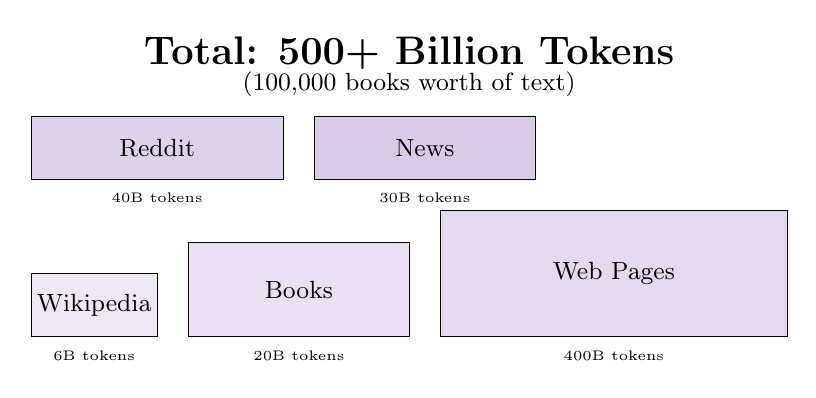
\begin{tikzpicture}[scale=0.8]
% Data sources with relative sizes
\draw[fill=mllavender!30] (0,0) rectangle (2,1);
\node at (1,0.5) {\small Wikipedia};
\node at (1,-0.3) {\tiny 6B tokens};

\draw[fill=mllavender!40] (2.5,0) rectangle (6,1.5);
\node at (4.25,0.75) {\small Books};
\node at (4.25,-0.3) {\tiny 20B tokens};

\draw[fill=mllavender!50] (6.5,0) rectangle (12,2);
\node at (9.25,1) {\small Web Pages};
\node at (9.25,-0.3) {\tiny 400B tokens};

\draw[fill=mllavender!60] (0,2.5) rectangle (4,3.5);
\node at (2,3) {\small Reddit};
\node at (2,2.2) {\tiny 40B tokens};

\draw[fill=mllavender!70] (4.5,2.5) rectangle (8,3.5);
\node at (6.25,3) {\small News};
\node at (6.25,2.2) {\tiny 30B tokens};

% Total
\node at (6,4.5) {\Large \textbf{Total: 500+ Billion Tokens}};
\node at (6,4) {\small (100,000 books worth of text)};
\end{tikzpicture}
\end{center}

\vspace{5mm}
\keypoint{Models read more in training than a human could in 10,000 lifetimes}

\bottomnote{GPT-3 trained on 45TB of compressed text}
\end{frame}

% Unsupervised Learning at Scale
\begin{frame}{Self-Supervised Learning: The Secret Sauce}
\textbf{How to create infinite training examples:}

\vspace{8mm}
\begin{columns}[T]
\column{0.48\textwidth}
\textbf{Method 1: Masked Language (BERT)}
\begin{enumerate}
\item Take: ``The cat sat on the mat``
\item Mask: ``The [MASK] sat on the mat``
\item Predict: ``cat``
\item Learn: Context → Word
\end{enumerate}

\vspace{5mm}
\textbf{Advantages:}
\begin{itemize}
\item Bidirectional context
\item Natural for understanding
\item Good for classification
\end{itemize}

\column{0.48\textwidth}
\textbf{Method 2: Next Word (GPT)}
\begin{enumerate}
\item Take: ``The cat sat on the``
\item Predict: ``mat``
\item Learn: Sequence → Next
\item Continue: Generate text
\end{enumerate}

\vspace{5mm}
\textbf{Advantages:}
\begin{itemize}
\item Natural generation
\item Autoregressive
\item Good for creation
\end{itemize}
\end{columns}

\vspace{8mm}
\keypoint{Both methods turn unlabeled text into labeled training data automatically}

\bottomnote{This self-supervision eliminates the annotation bottleneck}
\end{frame}

% Transfer Learning Theory
\begin{frame}{Transfer Learning: The Theory}
\textbf{Why does knowledge transfer work?}

\vspace{8mm}
\begin{center}
% \includegraphics[width=0.9\textwidth]{../figures/transfer_learning_landscape.pdf}
\textit{[Transfer learning landscape visualization]}
\end{center}

\vspace{5mm}
\textbf{Key insights:}
\begin{itemize}
\item \textbf{Lower layers}: Learn general features (word meanings, grammar)
\item \textbf{Middle layers}: Learn combinations (phrases, concepts)
\item \textbf{Upper layers}: Learn task-specific patterns
\item \textbf{Transfer}: Reuse lower/middle, adapt upper
\end{itemize}

\vspace{5mm}
\intuition{Like learning piano helps with typing - the finger coordination transfers}

\bottomnote{Neural networks naturally learn hierarchical representations}
\end{frame}

% The Pre-training Process
\begin{frame}{The Pre-training Process Workflow}
\textbf{From raw text to capable model:}

\vspace{5mm}
\begin{center}
\includegraphics[width=0.85\textwidth]{../figures/pretraining_workflow.pdf}
\end{center}

\vspace{5mm}
\textbf{Steps:}
\begin{enumerate}
\item \textbf{Collect}: Gather massive text corpus
\item \textbf{Clean}: Remove duplicates, filter quality
\item \textbf{Tokenize}: Convert text to tokens
\item \textbf{Create tasks}: Mask words or predict next
\item \textbf{Train}: Weeks on hundreds of GPUs
\item \textbf{Validate}: Check language understanding
\item \textbf{Release}: Share for community use
\end{enumerate}

\bottomnote{The entire process costs millions but happens only once}
\end{frame}

% What Models Actually Learn
\begin{frame}{Layers of Understanding: What Models Learn}
\textbf{Knowledge emerges at different depths:}

\vspace{8mm}
\begin{columns}[T]
\column{0.32\textwidth}
\textbf{Early Layers (1-4):}
\begin{itemize}
\item Character patterns
\item Word boundaries
\item Basic syntax
\item Parts of speech
\end{itemize}

\vspace{3mm}
\secondary{\small Example: ``run`` vs ``runs``}

\column{0.32\textwidth}
\textbf{Middle Layers (5-8):}
\begin{itemize}
\item Semantic meaning
\item Word relationships
\item Phrase structure
\item Dependencies
\end{itemize}

\vspace{3mm}
\secondary{\small Example: ``bank`` (river/money)}

\column{0.32\textwidth}
\textbf{Deep Layers (9-12):}
\begin{itemize}
\item Abstract concepts
\item Long-range patterns
\item Task-specific features
\item Reasoning steps
\end{itemize}

\vspace{3mm}
\secondary{\small Example: Inference, causality}
\end{columns}

\vspace{10mm}
\keypoint{Each layer builds on the previous - from letters to logic}

\bottomnote{Probing studies reveal this consistent hierarchy across models}
\end{frame}

% ============================================
% CHECKPOINT 1
% ============================================

\begin{frame}[t]{Checkpoint 1: Understanding Pre-training}
\begin{center}
\textbf{Test Your Understanding}
\end{center}
\vspace{5mm}

\begin{columns}[T]
\column{0.48\textwidth}
\textbf{Quick Quiz:}

\vspace{3mm}
\textbf{Q1:} What's the main advantage of pre-training?
\begin{itemize}
\item[A)] Faster inference
\item[B)] Transfer learning to any task
\item[C)] Smaller models
\item[D)] Less memory usage
\end{itemize}

\vspace{5mm}
\textbf{Q2:} How does self-supervision work?
\begin{itemize}
\item[A)] Humans label the data
\item[B)] Models label each other
\item[C)] Create labels from the text itself
\item[D)] Random labeling
\end{itemize}

\vspace{5mm}
\textbf{Q3:} Why is pre-training expensive but fine-tuning cheap?
\begin{itemize}
\item[A)] Different hardware
\item[B)] Pre-training learns general knowledge once
\item[C)] Fine-tuning uses less data
\item[D)] Both B and C
\end{itemize}

\column{0.48\textwidth}
\textbf{Answers:}

\vspace{3mm}
\textbf{A1:} B - Transfer learning to any task
\begin{itemize}
\item Pre-trained knowledge applies everywhere
\item One model bootstraps many applications
\item Eliminates starting from scratch
\end{itemize}

\vspace{5mm}
\textbf{A2:} C - Create labels from the text itself
\begin{itemize}
\item Mask words → predict them
\item Or predict next word
\item No human annotation needed
\end{itemize}

\vspace{5mm}
\textbf{A3:} D - Both B and C
\begin{itemize}
\item General knowledge learned once
\item Task-specific needs little data
\item 1000x less compute required
\end{itemize}
\end{columns}

\vspace{5mm}
\checkpoint{If you understand these concepts, you're ready to explore BERT and GPT!}
\end{frame}

% ============================================
% SECTION 3: THE ARCHITECTURE
% ============================================

\section{The Architecture: Two Paradigms}

% Section title slide
\begin{frame}
\begin{center}
{\Huge \textbf{Section 3}}\\
\vspace{5mm}
{\Large The Architecture}\\
\vspace{10mm}
{\large Two Paradigms: BERT and GPT}
\end{center}
\end{frame}

% BERT Introduction
\begin{frame}{BERT: Bidirectional Encoder Representations}
\textbf{The fill-in-the-blank master:}

\vspace{8mm}
\begin{columns}[T]
\column{0.48\textwidth}
\textbf{Core Idea:}
\begin{itemize}
\item Look at context from both sides
\item Mask random words (15\%)
\item Predict what's hidden
\item Learn deep bidirectional representations
\end{itemize}

\vspace{5mm}
\textbf{Architecture:}
\begin{itemize}
\item Transformer encoder only
\item 12/24 layers (Base/Large)
\item 110M/340M parameters
\item Attention in all directions
\end{itemize}

\column{0.48\textwidth}
\begin{center}
% \includegraphics[width=\textwidth]{../figures/bert_masking_visualization.pdf}
\textit{[BERT masking visualization]}
\end{center}

\vspace{3mm}
\textbf{Example:}\\
Input: ``The [MASK] sat on the [MASK]``\\
Output: ``cat``, ``mat`` (high probability)
\end{columns}

\vspace{8mm}
\intuition{BERT is like a detective examining all clues simultaneously to solve the mystery}

\bottomnote{BERT = Bidirectional Encoder Representations from Transformers}
\end{frame}

% Masked Language Modeling
\begin{frame}{Masked Language Modeling (MLM) Explained}
\textbf{How BERT learns from context:}

\vspace{8mm}
\begin{center}
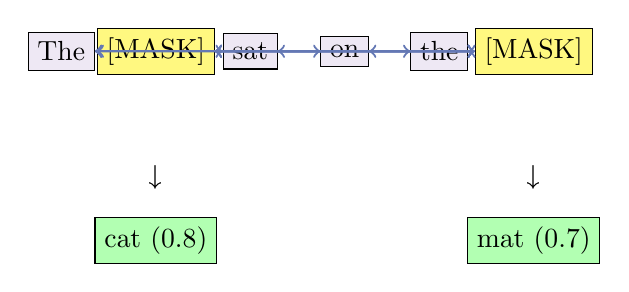
\begin{tikzpicture}[scale=0.8]
% Input sentence
\node[draw, fill=mllavender!30] (w1) at (0,3) {The};
\node[draw, fill=yellow!50] (w2) at (1.5,3) {[MASK]};
\node[draw, fill=mllavender!30] (w3) at (3,3) {sat};
\node[draw, fill=mllavender!30] (w4) at (4.5,3) {on};
\node[draw, fill=mllavender!30] (w5) at (6,3) {the};
\node[draw, fill=yellow!50] (w6) at (7.5,3) {[MASK]};

% Bidirectional arrows
\draw[<->, thick, mlblue] (w2) -- (w1);
\draw[<->, thick, mlblue] (w2) -- (w3);
\draw[<->, thick, mlblue] (w2) -- (w4);
\draw[<->, thick, mlblue] (w2) -- (w5);
\draw[<->, thick, mlblue] (w2) -- (w6);

\draw[<->, thick, mlblue] (w6) -- (w1);
\draw[<->, thick, mlblue] (w6) -- (w3);
\draw[<->, thick, mlblue] (w6) -- (w4);
\draw[<->, thick, mlblue] (w6) -- (w5);

% Predictions
\node at (1.5,1) {↓};
\node[draw, fill=green!30] at (1.5,0) {cat (0.8)};
\node at (7.5,1) {↓};
\node[draw, fill=green!30] at (7.5,0) {mat (0.7)};
\end{tikzpicture}
\end{center}

\vspace{8mm}
\textbf{Training details:}
\begin{itemize}
\item 80\% of masks: Replace with [MASK]
\item 10\% of masks: Replace with random word
\item 10\% of masks: Keep original (but still predict)
\end{itemize}

\keypoint{This prevents the model from only looking for [MASK] tokens}

\bottomnote{The 80-10-10 rule prevents overfitting to the [MASK] symbol}
\end{frame}

% GPT Introduction
\begin{frame}{GPT: Generative Pre-trained Transformer}
\textbf{The story continuation expert:}

\vspace{8mm}
\begin{columns}[T]
\column{0.48\textwidth}
\textbf{Core Idea:}
\begin{itemize}
\item Predict the next word
\item Use only left context
\item Autoregressive generation
\item Learn to continue any text
\end{itemize}

\vspace{5mm}
\textbf{Architecture:}
\begin{itemize}
\item Transformer decoder only
\item 12/24/48 layers (GPT/GPT-2/GPT-3)
\item 117M/1.5B/175B parameters
\item Causal (left-to-right) attention
\end{itemize}

\column{0.48\textwidth}
\begin{center}
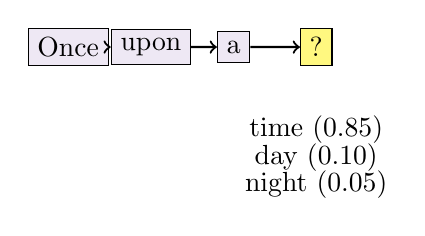
\begin{tikzpicture}[scale=0.7]
% Input sequence
\node[draw, fill=mllavender!30] (w1) at (0,2) {Once};
\node[draw, fill=mllavender!30] (w2) at (1.5,2) {upon};
\node[draw, fill=mllavender!30] (w3) at (3,2) {a};
\node[draw, fill=yellow!50] (w4) at (4.5,2) {?};

% Arrows showing causal flow
\draw[->, thick] (w1) -- (w2);
\draw[->, thick] (w2) -- (w3);
\draw[->, thick] (w3) -- (w4);

% Predictions
\node at (4.5,0.5) {time (0.85)};
\node at (4.5,0) {day (0.10)};
\node at (4.5,-0.5) {night (0.05)};
\end{tikzpicture}
\end{center}

\vspace{3mm}
\textbf{Example:}\\
Input: ``Once upon a``\\
Output: ``time`` (highest probability)
\end{columns}

\vspace{8mm}
\intuition{GPT is like an author who can only see what's been written so far}

\bottomnote{GPT = Generative Pre-trained Transformer}
\end{frame}

% Causal Language Modeling
\begin{frame}{Causal Language Modeling Explained}
\textbf{How GPT learns to generate:}

\vspace{8mm}
\begin{columns}[T]
\column{0.48\textwidth}
\textbf{Training Process:}
\begin{enumerate}
\item Start with text sequence
\item Predict each word from previous
\item Compare with actual next word
\item Update to improve predictions
\end{enumerate}

\vspace{5mm}
\textbf{Attention Mask:}
\begin{center}
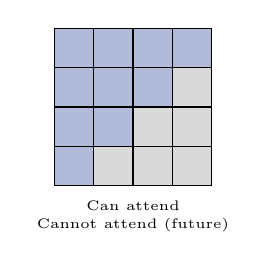
\begin{tikzpicture}[scale=0.5]
% Attention matrix
\draw[fill=mlblue!50] (0,0) rectangle (1,1);
\draw[fill=mlblue!50] (0,1) rectangle (1,2);
\draw[fill=mlblue!50] (0,2) rectangle (1,3);
\draw[fill=mlblue!50] (0,3) rectangle (1,4);

\draw[fill=gray!30] (1,0) rectangle (2,1);
\draw[fill=mlblue!50] (1,1) rectangle (2,2);
\draw[fill=mlblue!50] (1,2) rectangle (2,3);
\draw[fill=mlblue!50] (1,3) rectangle (2,4);

\draw[fill=gray!30] (2,0) rectangle (3,1);
\draw[fill=gray!30] (2,1) rectangle (3,2);
\draw[fill=mlblue!50] (2,2) rectangle (3,3);
\draw[fill=mlblue!50] (2,3) rectangle (3,4);

\draw[fill=gray!30] (3,0) rectangle (4,1);
\draw[fill=gray!30] (3,1) rectangle (4,2);
\draw[fill=gray!30] (3,2) rectangle (4,3);
\draw[fill=mlblue!50] (3,3) rectangle (4,4);

\node at (2,-0.5) {\tiny Can attend};
\node at (2,-1) {\tiny Cannot attend (future)};
\end{tikzpicture}
\end{center}

\column{0.48\textwidth}
\textbf{Generation Process:}
\begin{enumerate}
\item Start with prompt
\item Generate next token
\item Add to sequence
\item Repeat until done
\end{enumerate}

\vspace{5mm}
\textbf{Example Generation:}
\begin{itemize}
\item Prompt: ``The weather``
\item Step 1: ``The weather \textbf{is}``
\item Step 2: ``The weather is \textbf{nice}``
\item Step 3: ``The weather is nice \textbf{today}``
\end{itemize}
\end{columns}

\vspace{8mm}
\keypoint{Causal masking ensures the model can't cheat by looking ahead}

\bottomnote{This autoregressive property enables open-ended generation}
\end{frame}

% BERT vs GPT Comparison
\begin{frame}{BERT vs GPT: Head-to-Head Comparison}
\textbf{Two paradigms, different strengths:}

\vspace{5mm}
\begin{center}
\includegraphics[width=0.8\textwidth]{../figures/bert_vs_gpt_architecture.pdf}
\end{center}

\vspace{5mm}
\begin{center}
\begin{tabular}{|l|c|c|}
\hline
\textbf{Aspect} & \textbf{BERT} & \textbf{GPT} \\
\hline
Context & Bidirectional & Left-to-right only \\
Best for & Understanding & Generation \\
Training & Masked LM & Next token prediction \\
Architecture & Encoder only & Decoder only \\
Fine-tuning & Required & Optional (few-shot) \\
Use cases & Classification, QA & Text generation, completion \\
\hline
\end{tabular}
\end{center}

\vspace{5mm}
\keypoint{Choose BERT for analysis, GPT for creation}

\bottomnote{Modern models like T5 combine both approaches}
\end{frame}

% When to Use Which
\begin{frame}{Choosing the Right Approach}
\textbf{Decision tree for model selection:}

\vspace{8mm}
\begin{center}
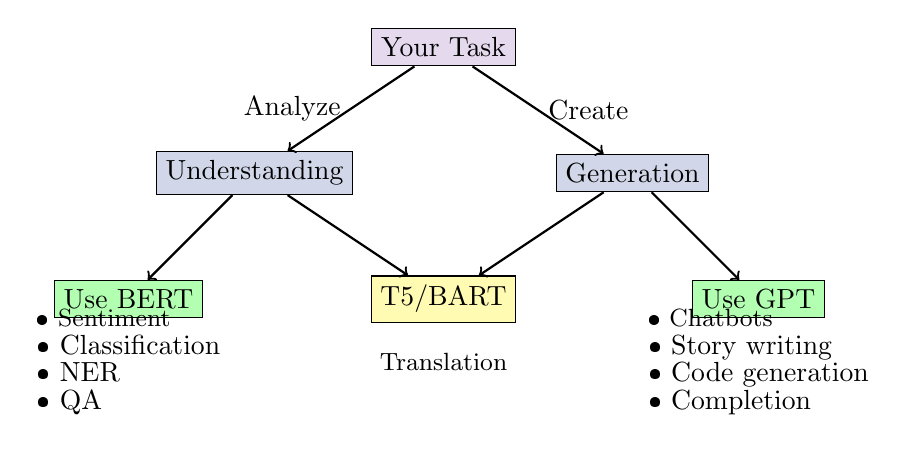
\begin{tikzpicture}[scale=0.8]
% Root
\node[draw, fill=mllavender!50] (root) at (0,0) {Your Task};

% First split
\node[draw, fill=mlblue!30] (understand) at (-3,-2) {Understanding};
\node[draw, fill=mlblue!30] (generate) at (3,-2) {Generation};

\draw[->, thick] (root) -- (understand) node[midway, left] {Analyze};
\draw[->, thick] (root) -- (generate) node[midway, right] {Create};

% BERT branch
\node[draw, fill=green!30] (bert) at (-5,-4) {Use BERT};
\node[align=left] at (-5,-5) {\small • Sentiment\\[-2pt] • Classification\\[-2pt] • NER\\[-2pt] • QA};

\draw[->, thick] (understand) -- (bert);

% GPT branch
\node[draw, fill=green!30] (gpt) at (5,-4) {Use GPT};
\node[align=left] at (5,-5) {\small • Chatbots\\[-2pt] • Story writing\\[-2pt] • Code generation\\[-2pt] • Completion};

\draw[->, thick] (generate) -- (gpt);

% Hybrid
\node[draw, fill=yellow!30] (hybrid) at (0,-4) {T5/BART};
\node at (0,-5) {\small Translation};

\draw[->, thick] (understand) -- (hybrid);
\draw[->, thick] (generate) -- (hybrid);
\end{tikzpicture}
\end{center}

\vspace{8mm}
\realworld{Google uses BERT for search understanding, OpenAI uses GPT for ChatGPT}

\bottomnote{Most real applications use task-appropriate architectures}
\end{frame}

% ============================================
% CHECKPOINT 2
% ============================================

\begin{frame}[t]{Checkpoint 2: BERT vs GPT Understanding}
\begin{center}
\textbf{Test Your Architecture Knowledge}
\end{center}
\vspace{5mm}

\begin{columns}[T]
\column{0.48\textwidth}
\textbf{Architecture Quiz:}

\vspace{3mm}
\textbf{Q1:} Why can't BERT generate text well?
\begin{itemize}
\item[A)] Too small
\item[B)] Bidirectional training
\item[C)] Wrong architecture
\item[D)] Not enough data
\end{itemize}

\vspace{5mm}
\textbf{Q2:} What makes GPT good at generation?
\begin{itemize}
\item[A)] Larger size
\item[B)] Autoregressive training
\item[C)] Better data
\item[D)] Faster inference
\end{itemize}

\vspace{5mm}
\textbf{Q3:} For sentiment analysis, which is better?
\begin{itemize}
\item[A)] GPT - generates sentiment
\item[B)] BERT - understands full context
\item[C)] Either works equally
\item[D)] Need both together
\end{itemize}

\column{0.48\textwidth}
\textbf{Answers:}

\vspace{3mm}
\textbf{A1:} B - Bidirectional training
\begin{itemize}
\item BERT sees future context during training
\item Can't generate sequentially
\item Designed for understanding, not creation
\end{itemize}

\vspace{5mm}
\textbf{A2:} B - Autoregressive training
\begin{itemize}
\item Learns to predict next token
\item Natural for sequential generation
\item Each output becomes next input
\end{itemize}

\vspace{5mm}
\textbf{A3:} B - BERT understands full context
\begin{itemize}
\item Sees entire sentence at once
\item Better for classification tasks
\item GPT only sees left context
\end{itemize}
\end{columns}

\vspace{5mm}
\checkpoint{Understanding these differences is crucial for choosing the right model}
\end{frame}

% ============================================
% SECTION 4: THE REVOLUTION
% ============================================

\section{The Revolution: From Pre-training to Your Task}

% Section title slide
\begin{frame}
\begin{center}
{\Huge \textbf{Section 4}}\\
\vspace{5mm}
{\Large The Revolution}\\
\vspace{10mm}
{\large From Pre-training to Your Task}
\end{center}
\end{frame}

% Fine-tuning Introduction
\begin{frame}{Fine-tuning: Teaching New Tricks}
\textbf{Adapting general knowledge to specific tasks:}

\vspace{8mm}
\begin{columns}[T]
\column{0.48\textwidth}
\textbf{The Process:}
\begin{enumerate}
\item Start with pre-trained model
\item Add task-specific head
\item Train on your labeled data
\item Much less data needed (100s-1000s)
\item 10-100x faster than from scratch
\end{enumerate}

\vspace{5mm}
\textbf{What changes:}
\begin{itemize}
\item Top layers adapt most
\item Lower layers change little
\item Task head learns mapping
\end{itemize}

\column{0.48\textwidth}
\begin{center}
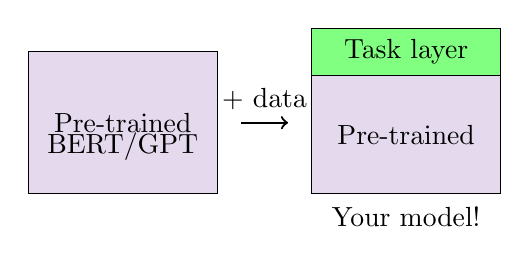
\begin{tikzpicture}[scale=0.6]
% Pre-trained model
\draw[fill=mllavender!50] (0,0) rectangle (4,3);
\node at (2,1.5) {Pre-trained};
\node at (2,1) {BERT/GPT};

% Arrow
\draw[->, thick] (4.5,1.5) -- (5.5,1.5);
\node at (5,2) {+ data};

% Fine-tuned model
\draw[fill=mllavender!50] (6,0) rectangle (10,2.5);
\draw[fill=green!50] (6,2.5) rectangle (10,3.5);
\node at (8,1.25) {Pre-trained};
\node at (8,3) {Task layer};

% Results
\node at (8,-0.5) {Your model!};
\end{tikzpicture}
\end{center}

\vspace{8mm}
\textbf{Example - Sentiment Analysis:}
\begin{itemize}
\item Pre-trained BERT: Knows language
\item Your data: 1000 movie reviews
\item Fine-tune: 1 hour on 1 GPU
\item Result: 95\% accuracy
\end{itemize}
\end{columns}

\vspace{5mm}
\keypoint{Fine-tuning is like teaching a PhD student - they already know how to learn}

\bottomnote{Most production NLP systems are fine-tuned pre-trained models}
\end{frame}

% The Model Zoo
\begin{frame}{The Model Zoo: Choose Your Fighter!}
\textbf{Pre-trained models available today:}

\vspace{8mm}
\begin{center}
\begin{tabular}{|l|c|c|c|c|}
\hline
\textbf{Model} & \textbf{Size} & \textbf{Type} & \textbf{Best For} & \textbf{Company} \\
\hline
BERT-base & 110M & Encoder & Classification & Google \\
BERT-large & 340M & Encoder & Understanding & Google \\
RoBERTa & 355M & Encoder & Robust tasks & Facebook \\
\hline
GPT-2 & 1.5B & Decoder & Generation & OpenAI \\
GPT-3 & 175B & Decoder & Few-shot & OpenAI \\
GPT-4 & ~1T & Decoder & Everything & OpenAI \\
\hline
T5 & 11B & Enc-Dec & Text-to-text & Google \\
BART & 400M & Enc-Dec & Summarization & Facebook \\
mT5 & 13B & Enc-Dec & Multilingual & Google \\
\hline
\end{tabular}
\end{center}

\vspace{8mm}
\realworld{HuggingFace hosts 100,000+ pre-trained models ready to use}

\bottomnote{The model zoo grows daily - new models appear weekly}
\end{frame}

% Implementation with HuggingFace
\begin{frame}[fragile]{Using Pre-trained Models in Practice}
\textbf{5 lines of code to state-of-the-art:}

\vspace{5mm}
\begin{lstlisting}[language=Python]
from transformers import pipeline

# Load pre-trained model
classifier = pipeline(``sentiment-analysis``)

# Use immediately
result = classifier(``I love this movie!``)
# Output: [{'label': 'POSITIVE', 'score': 0.999}]

# Or fine-tune on your data
from transformers import AutoModelForSequenceClassification, Trainer

model = AutoModelForSequenceClassification.from_pretrained(``bert-base``)
trainer = Trainer(model=model, train_dataset=your_data)
trainer.train()  # Fine-tunes in hours, not weeks
\end{lstlisting}

\vspace{5mm}
\keypoint{Modern libraries make pre-trained models as easy as importing a package}

\bottomnote{HuggingFace Transformers is the standard library for pre-trained models}
\end{frame}

% Model Selection Decision Tree
\begin{frame}[fragile]{Which Model Should You Use?}
\textbf{Practical decision guide:}

\vspace{8mm}
\begin{columns}[T]
\column{0.48\textwidth}
\textbf{Start with these questions:}
\begin{enumerate}
\item What's your task?
\begin{itemize}
\item Classification → BERT/RoBERTa
\item Generation → GPT-2/GPT-3
\item Translation → T5/mT5
\end{itemize}
\item How much data do you have?
\begin{itemize}
\item $<$100 examples → GPT-3 few-shot
\item 100-1000 → Fine-tune small model
\item $>$1000 → Fine-tune large model
\end{itemize}
\item What's your budget?
\begin{itemize}
\item Free → BERT-base
\item \$100s → GPT-2
\item \$1000s → GPT-3 API
\end{itemize}
\end{enumerate}

\column{0.48\textwidth}
\textbf{Model size vs performance:}
\begin{center}
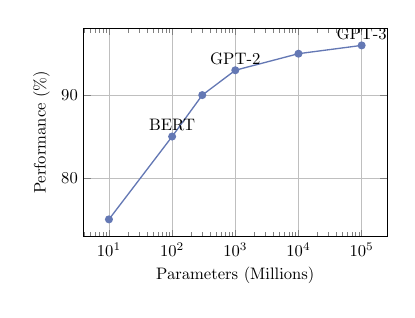
\begin{tikzpicture}[scale=0.6]
\begin{axis}[
    xlabel={Parameters (Millions)},
    ylabel={Performance (\%)},
    width=8cm,
    height=6cm,
    xmode=log,
    grid=major
]
\addplot[color=mlblue, thick, mark=*] coordinates {
    (10, 75)
    (100, 85)
    (300, 90)
    (1000, 93)
    (10000, 95)
    (100000, 96)
};
\node at (axis cs:100,85) [above] {BERT};
\node at (axis cs:1000,93) [above] {GPT-2};
\node at (axis cs:100000,96) [above] {GPT-3};
\end{axis}
\end{tikzpicture}
\end{center}

\textbf{Diminishing returns:}\\
10x size → 2-3\% improvement
\end{columns}

\vspace{8mm}
\misconception{``Bigger is always better'' - False! BERT-base beats GPT-3 on many specific tasks}

% Note: Start small, scale up only if needed
\end{frame}

% Evolution Timeline
\begin{frame}{The Evolution: From ELMo to GPT-4}
\textbf{How we got here:}

\vspace{8mm}
\begin{center}
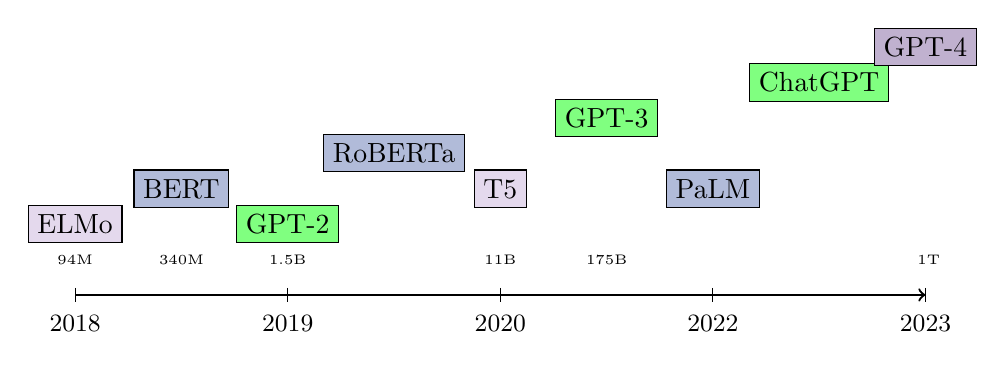
\begin{tikzpicture}[scale=0.9]
% Timeline
\draw[thick, ->] (0,0) -- (12,0);

% Years
\foreach \x/\year in {0/2018, 3/2019, 6/2020, 9/2022, 12/2023} {
    \draw (\x,0.1) -- (\x,-0.1);
    \node at (\x,-0.4) {\small \year};
}

% Models
\node[draw, fill=mllavender!50] at (0,1) {ELMo};
\node[draw, fill=mlblue!50] at (1.5,1.5) {BERT};
\node[draw, fill=green!50] at (3,1) {GPT-2};
\node[draw, fill=mlblue!50] at (4.5,2) {RoBERTa};
\node[draw, fill=mllavender!50] at (6,1.5) {T5};
\node[draw, fill=green!50] at (7.5,2.5) {GPT-3};
\node[draw, fill=mlblue!50] at (9,1.5) {PaLM};
\node[draw, fill=green!50] at (10.5,3) {ChatGPT};
\node[draw, fill=mlpurple!50] at (12,3.5) {GPT-4};

% Size annotations
\node at (0,0.5) {\tiny 94M};
\node at (1.5,0.5) {\tiny 340M};
\node at (3,0.5) {\tiny 1.5B};
\node at (6,0.5) {\tiny 11B};
\node at (7.5,0.5) {\tiny 175B};
\node at (12,0.5) {\tiny ~1T};
\end{tikzpicture}
\end{center}

\vspace{8mm}
\textbf{Key milestones:}
\begin{itemize}
\item \textbf{2018}: Pre-training idea proven (ELMo, BERT)
\item \textbf{2019}: Scale begins (GPT-2 ``too dangerous to release``)
\item \textbf{2020}: Few-shot learning (GPT-3)
\item \textbf{2022}: Instruction following (ChatGPT)
\item \textbf{2023}: Multimodal understanding (GPT-4)
\end{itemize}

\bottomnote{5 years from research to changing the world}
\end{frame}

% Real-world Impact
\begin{frame}{Real-world Applications and Impact}
\textbf{Pre-trained models in production:}

\vspace{8mm}
\begin{columns}[T]
\column{0.32\textwidth}
\textbf{Search \& QA:}
\begin{itemize}
\item Google Search (BERT)
\item Bing (GPT-4)
\item Stack Overflow
\item Customer support
\end{itemize}

\vspace{3mm}
\secondary{\small 10B+ queries daily}

\column{0.32\textwidth}
\textbf{Content Creation:}
\begin{itemize}
\item GitHub Copilot
\item Copy.ai
\item Jasper
\item ChatGPT
\end{itemize}

\vspace{3mm}
\secondary{\small \$1B+ market}

\column{0.32\textwidth}
\textbf{Understanding:}
\begin{itemize}
\item Gmail Smart Reply
\item Grammarly
\item Translation
\item Medical diagnosis
\end{itemize}

\vspace{3mm}
\secondary{\small 1B+ users}
\end{columns}

\vspace{10mm}
\begin{center}
\colorbox{green!20}{
\parbox{0.8\textwidth}{
\centering
\textbf{Impact: Every text you read online has likely been processed by a pre-trained model}
}
}
\end{center}

\bottomnote{Pre-trained models are the foundation of modern AI applications}
\end{frame}

% The Future
\begin{frame}{The Future: What's Next?}
\textbf{Where pre-training is heading:}

\vspace{8mm}
\begin{columns}[T]
\column{0.48\textwidth}
\textbf{Current Trends:}
\begin{itemize}
\item \textbf{Multimodal}: Text + Images + Audio
\item \textbf{Longer context}: 100K+ tokens
\item \textbf{Efficiency}: Same performance, 10x smaller
\item \textbf{Specialization}: Domain-specific models
\item \textbf{Personalization}: Models that know you
\end{itemize}

\vspace{5mm}
\textbf{Challenges:}
\begin{itemize}
\item Computational cost
\item Data quality
\item Hallucination
\item Bias and fairness
\end{itemize}

\column{0.48\textwidth}
\textbf{Emerging Capabilities:}
\begin{itemize}
\item Reasoning and planning
\item Tool use and APIs
\item Self-correction
\item Continuous learning
\item Uncertainty awareness
\end{itemize}

\vspace{5mm}
\textbf{Next 5 Years:}
\begin{itemize}
\item Personal AI assistants
\item Scientific discovery
\item Creative partners
\item Educational tutors
\item Medical advisors
\end{itemize}
\end{columns}

\vspace{8mm}
\keypoint{We're moving from ``models that know language`` to ``models that understand the world``}

\bottomnote{The pre-training paradigm will likely evolve but not disappear}
\end{frame}

% Key Takeaways
\begin{frame}{Key Takeaways: What to Remember}
\begin{center}
{\Large \textbf{The Pre-training Revolution}}
\end{center}

\vspace{10mm}
\begin{enumerate}
\item \textbf{The Problem:} Everyone was learning language from scratch
\vspace{3mm}
\item \textbf{The Solution:} Pre-train once, fine-tune many times
\vspace{3mm}
\item \textbf{The Methods:}
\begin{itemize}
\item BERT: Bidirectional understanding (fill-in-blanks)
\item GPT: Autoregressive generation (predict next)
\end{itemize}
\vspace{3mm}
\item \textbf{The Impact:}
\begin{itemize}
\item 100x faster development
\item 10x cost reduction
\item Better performance
\end{itemize}
\vspace{3mm}
\item \textbf{The Practice:} Use HuggingFace, start small, scale if needed
\vspace{3mm}
\item \textbf{The Future:} Multimodal, efficient, personalized
\end{enumerate}

\vspace{10mm}
\keypoint{Pre-training democratized NLP - anyone can now build SOTA models}

\bottomnote{You now understand the technology behind ChatGPT, BERT, and modern AI}
\end{frame}

% Summary
\begin{frame}{Summary: From Zero to Hero}
\textbf{Your journey today:}

\vspace{10mm}
\begin{columns}[T]
\column{0.48\textwidth}
\textbf{The Challenge:}
\begin{itemize}
\item Wasteful repetition
\item \$10M problem
\item Environmental impact
\item Starting from scratch
\end{itemize}

\vspace{8mm}
\textbf{The Foundation:}
\begin{itemize}
\item Self-supervised learning
\item Transfer learning theory
\item Learning from internet
\item Hierarchical knowledge
\end{itemize}

\column{0.48\textwidth}
\textbf{The Architecture:}
\begin{itemize}
\item BERT for understanding
\item GPT for generation
\item Choose based on task
\item Both have strengths
\end{itemize}

\vspace{8mm}
\textbf{The Revolution:}
\begin{itemize}
\item Fine-tuning magic
\item Model zoo available
\item 5 lines to SOTA
\item Changed everything
\end{itemize}
\end{columns}

\vspace{10mm}
\keypoint{You now understand pre-training - the foundation of modern NLP!}

\bottomnote{Next week: Advanced transformer architectures and techniques}
\end{frame}

% Final slide
\begin{frame}
\begin{center}
{\Huge \textbf{Thank You!}}\\
\vspace{10mm}
{\Large Questions?}\\
\vspace{15mm}
{\large Next: Lab Session - Fine-tuning BERT}\\
\vspace{5mm}
\secondary{\footnotesize We'll fine-tune BERT for sentiment analysis in 30 minutes}
\end{center}
\end{frame}

\end{document}